%%
% Please see https://bitbucket.org/rivanvx/beamer/wiki/Home for obtaining beamer.
%%
%\documentclass[11pt,aspectratio=169]{beamer}
%\documentclass[11pt,aspectratio=169,xcolor={dvipsnames}]{beamer}

\documentclass[11pt,aspectratio=169,xcolor={dvipsnames},hyperref={pdftex,pdfpagemode=UseNone,hidelinks,pdfdisplaydoctitle=true},usepdftitle=false]{beamer}
\usepackage{presentation}


\title{Lecture 14: The Financial Accelerator}
\author{Juan Herre\~{n}o\\UCSD}
\date{2026}

% Enter presentation title to populate PDF metadata:
\newcommand{\Cov}{\text{Cov}_\lambda}
\newcommand{\El}{\mathbb{E}_\lambda}
\newcommand{\mm}{\text{{\fontfamily{qzc}\selectfont m}}}
\usepackage{cancel}
\usepackage{booktabs}
\begin{document}

\maketitle


\begin{frame}{Goal for Today}
 We want to capture the following narrative of booms and busts
\begin{itemize}
\item In good times
\begin{itemize}
\item In good times it is easier for firms to access funding
\item So they can invest more
\item This expands output and makes funding even easier to access
\end{itemize}
\item In bad times
\begin{itemize}
\item It is harder for firms to access debt
\item Curtailing the ability of firms to invest
\item Which reduces the capital stock in the future, and depresses production
\item Doom loop.	
\end{itemize}
\end{itemize}
We will plug our Costly State Verification model into a stripped-down version of the RBC model for simplicity
\end{frame}
%\begin{frame}
%\begin{itemize}
%\item Follows Steinsson's lecture notes
%\item Treatment follows Romer 2019
%\end{itemize}
%\end{frame}

\begin{frame}{Messages from CSV Models}
Last lecture
\begin{itemize}
\item Asymmetric Information problem between borrowers and savers
\item Think of borrowers as firms
\item Think of lenders as banks
\item Could write similar model between banks and bond-holders
\end{itemize}
This lecture
\begin{itemize}
\item Relax the assumption of a fixed $r$ and fixed $W$
\item Amplification of financial frictions with the business cycle
\item Following Bernanke Gertler (1989)
\end{itemize}
\end{frame}

\begin{frame}{Setting}
Standard RBC model (As in 210A) with financial frictions
\begin{itemize}
\item A production function with TFP shocks, lowercase variables in per-capita terms
\[y_t = \tilde{\theta}_t f(k_t) \]
\item with the non-standard assumption that $f(0) > 0 $
\item Investment technologies take $t$ output and transform it into $t+1$ capital
\item Two types of agents: entrepreneurs and lenders. $\eta$ is the share of entrepreneurs
\item Heterogeneous entrepreneurs, homogeneous lenders
\item OLG model: Young, old, exit. Think of an agent as a project that needs funding
\end{itemize}
\end{frame}

\begin{frame}{Entrepreneurs and Capital Accumulation}
\begin{itemize}
\item Only \textit{entrepreneurs} have investment technologies.
\item Entrepreneurs come in types $\omega \sim U[0,1]$
\item Input: Entrepreneur of type $\omega$ uses $x(\omega)$ units of output exactly to produce capital
\item Result: $\kappa_i$ units of capital, where  $i = 1,..,n$ with $\kappa_j \geq \kappa_k$ whenever $j > k$, probabilities $\pi_i$.
\item $\mathbb{E} \kappa_i = \kappa$
\item $\kappa$ uncorrelated with $\omega$
\item Whenever the economy needs more capital, more entrepreneurs will be active...
\item The marginal entrepreneur will be worse than the average entrepreneur
\item So the supply curve of capital will be upward sloping
\end{itemize}
\end{frame}

\begin{frame}{Information}
\begin{itemize}
\item The realization $\kappa_i$ is the private information of the entrepreneur
\item Lenders have a unique auditing technology that absorbs $\gamma$ units of capital
\item When used, it reveals the outcome with probability 1
\item Timing:
\begin{itemize}
\item $\kappa$'s are realized, owners announce $\tilde{\kappa}$, auditing takes place, then $\tilde{\theta}$ is realized
\item Law of motion of capital
\[k_{t+1} = (\kappa - h_t \gamma) i_t\]
\item $k, i, h$ endogenous
\end{itemize}
\end{itemize}
\end{frame}

\begin{frame}{Savings}
\begin{itemize}
\item OLG setting + risk neutrality wrt $t+1$ consumption
\item Savings
\begin{itemize}
\item Entrepreneur: $S^e_t = w_t L^e_t$
\item Lenders: $S_t = w_t L - z^*_y(r)$
\end{itemize}
\item Link between savings and wage rates.
\item Note: assumptions such that savings > investment, so that the marginal return on savings is $r$, the return on an outside option inventory holding technology
\end{itemize}
\end{frame}

\begin{frame}{Perfect Information}
Case with $\gamma = 0$. 
\begin{itemize}
\item Indifference condition (in expectation) pins down the marginal entrepreneur $\bar{\omega}$
\[\hat{q}_{t+1} \kappa - r x(\bar{\omega}) = 0\]
\item $\hat{q}_{t+1}$ is the expected price of capital tomorrow
\item Everybody with $\omega < \bar{\omega}$ operates their technology 
\item Savings exceed investment demand by assumption (marginal return = $r$)
\[\eta S^e_t + (1-\eta)S_t > \int_0^{\bar{\omega}} x(\omega) d\omega\]
\item $i_t = \bar{\omega} \eta$ and $k_{t+1} = \kappa i_t$, so that the capital supply curve:
\[\hat{q}_{t+1} =  r x\left(\frac{k_{t+1}}{\kappa \eta} \right) /\kappa \]
\end{itemize}
\end{frame}

\begin{frame}{Perfect Information}
Case with $\gamma = 0$. 
\begin{itemize}
\item Capital supply curve:
\[\hat{q}_{t+1} =  r x\left(\frac{k_{t+1}}{\kappa \eta} \right) /\kappa \]
\item Capital demand curve
\[\hat{q}_{t+1} = \theta f'(k_{t+1}) \]
\item The intersection of supply and demand is independent from period $t$ variables
\[\hat{q}_{t+1} = q\] \[k_{t+1} = k\]
\item Feature:  $i = \bar{\omega} \eta$, because $\bar{\omega}$ is constant due to $\hat{q}$ being constant
\end{itemize}
\end{frame}


\begin{frame}{Asymmetric Information}
Case with $\gamma > 0$
\begin{itemize}
\item Objective: Maximize entrepreneurs consumption
\[ \max \pi_1(p c^a + (1-p)c_1) +\pi_2 c_2\]
\item Subject to:
\begin{itemize}
\item Participation constraint on the lenders (funding the project is better than saving in inventories)
\[\pi_1 (\hat{q}\kappa_1 - (1-p) c_1 - p(c^a + \gamma \hat{q}) )+ \pi_2 (\hat{q} \kappa_2 - c_2) \geq r(x - S^e) \]
\item IC constraint (announcing the good state is preferable to lie, and sell the excess capital in the market)
\[c_2 \geq p(0) + (1-p) (c_1 + (\kappa_2 - \kappa_1) \hat{q}) \]
\item Limited liability + feasibility constraint
 \[c_1 \geq 0, c^a \geq 0, 0 \leq p \leq 1\]
\end{itemize}
\end{itemize}
\end{frame}

\begin{frame}{Two Regimes with $n=2$ states}
\begin{itemize}
\item Case 1: The entrepreneur is sufficiently wealthy (full collateralization)
\begin{itemize}
	\item Even if the bad state materializes $\hat{q} \kappa_1 \geq r(x(\omega) - S^e)$
	\item No agency costs (distribution of states is public info)
\end{itemize}
\item $\hat{q} \kappa_1 < r(x(\omega) - S^e)$ (incomplete collateralization)
\begin{itemize}
	\item Optimal auditing probability
	\[ p(\omega) = \frac{r(x(\omega) - S^e) - \hat{q} \kappa_1}{\pi_2 \hat{q}(\kappa_2  - \kappa_1) - \pi_1 \hat{q}\gamma} \]
	\item (comes from setting every constraint with equality)
\end{itemize}
\end{itemize}
In the full collateralization case, outside finance is provided at rate $r$ (no risk)
\end{frame}

\begin{frame}{Good entrepreneur}
\begin{figure}
\centering
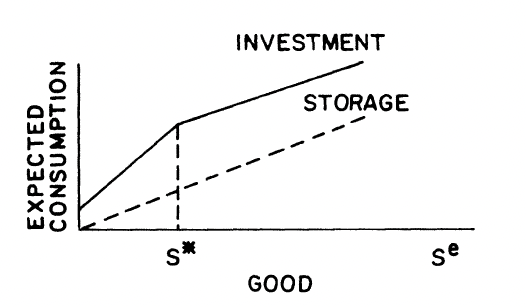
\includegraphics[scale=0.5]{FiguresTables/bg_1}
\end{figure}
consumption rises faster than slope $r$ (dotted line) since financial costs decrease with wealth
\end{frame}

\begin{frame}{Bad entrepreneur}
\begin{figure}
\centering
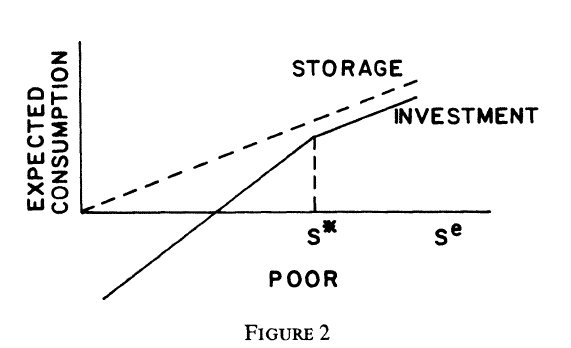
\includegraphics[scale=0.5]{FiguresTables/bg_2}
\end{figure}
\end{frame}


\begin{frame}{Fair entrepreneur}
\begin{figure}
\centering
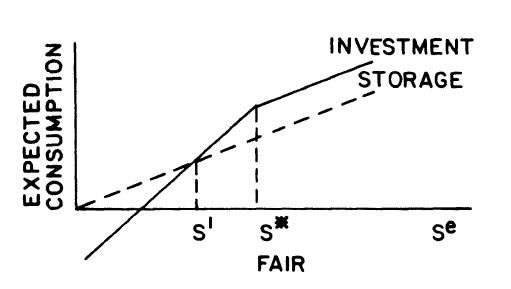
\includegraphics[scale=0.5]{FiguresTables/bg_3}
\end{figure}
Convex envelope between 0 and $S^*$. These entrepreneurs will enter a lottery (how realistic?). For given $\omega$ they will enter a lottery that pays $S^*$ with probability $g(\omega) = S^e/S(\omega)^*$
\end{frame}

\begin{frame}{Capital Supply}
\begin{itemize}
\item Aggregate Capital tomorrow
\[k_{t+1} =\eta \left[ \kappa \underline{\omega}  - \pi_1 \gamma \int_0^{\underline{\omega}} p(\omega) d\omega + \kappa \int_{\underline{\omega}}^{\bar{\omega}} g(\omega) d\omega \right] \]
\item Can be rewritten as:
\[k_{t+1} =\eta \left[ \kappa \bar{\omega}  -  \int_0^{\underline{\omega}} \pi_1 \gamma p(\omega) d\omega - \int_{\underline{\omega}}^{\bar{\omega}} \kappa(1-g(\omega) )d\omega \right] \]


\item $\underline{\omega}$, $\bar{\omega}$, $p(\omega)$, $g(\omega)$ are all functions of $q$.
\item This equation is the supply curve of capital (with $d k_{t+1}/ d\hat{q}_{t+1} > 0)$
\item Problem set question: Prove  $d k_{t+1}/ d\hat{q}_{t+1} > 0$
\end{itemize}
\end{frame}

\begin{frame}{Some Properties of Capital Supply}
\[k_{t+1} =\eta \left[ \kappa \bar{\omega}  -  \int_0^{\underline{\omega}} \pi_1 \gamma p(\omega) d\omega - \int_{\underline{\omega}}^{\bar{\omega}} \kappa(1-g(\omega) )d\omega \right] \]
\begin{itemize}
\item The supply schedule is to the left of the FI supply
\[k_{t+1} \leq \kappa \bar{\omega} \eta\]
\item For sufficiently large $(k_{t+1},\hat{q}_{t+1})$, the AI and FI schedules coincide
\begin{itemize}
\item $p(\omega) \rightarrow 0$, and $g(\omega) \rightarrow 1$.
\end{itemize}
\item $t+1$ outcomes depend on  $t$ variables
	\[ p(\omega) = \frac{r(x(\omega) - S^e) - \hat{q} \kappa_1}{\pi_2 \hat{q}(\kappa_2  - \kappa_1) - \pi_1 \hat{q}\gamma} \]
\end{itemize}
\end{frame}

\begin{frame}{Supply and Demand of Capital}
\begin{figure}
\centering
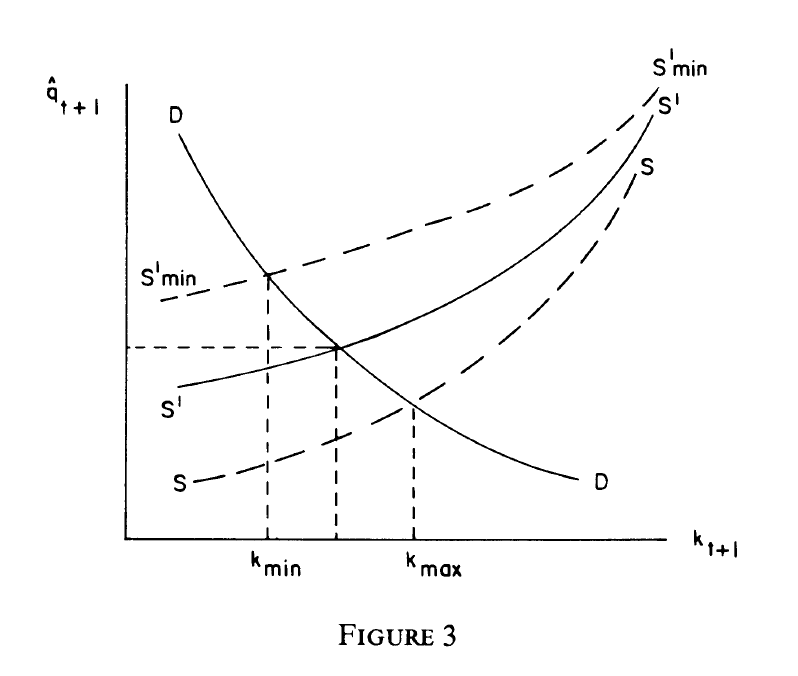
\includegraphics[scale=0.6]{FiguresTables/bg_4}
\end{figure}
Notice the demand of capital is given by $\hat{q}_{t+1} = \theta f'(k_{t+1})$
\end{frame}

\begin{frame}{Accelerator}
\begin{itemize}
\item Imagine a negative shock that drives down savings (via labor income for example)
\item Lower wealth increases agency problems $\rightarrow$ $\uparrow p$
\item Increases inspection costs
\begin{itemize}
\item Shifts capital supply to the left
\item Financed projects become more costly to finance
\item Less projects are financed
\end{itemize}
\item Lower investment, and capital tomorrow
\item Less production tomorrow, and lower savings. Doom loop.
\end{itemize}
Persistent investment slumps in which financing and producing capital is costly
\end{frame}



\end{document}




